\documentclass{standalone}

\usepackage{tikz}

\begin{document}

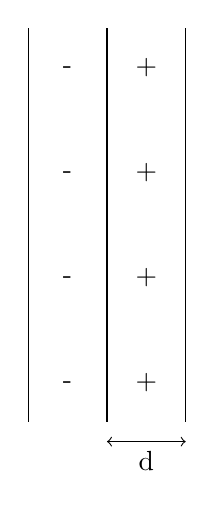
\begin{tikzpicture}

	\def\h{5} % Hauteur de la sheet
	
	\def\d{1} % Distance entre les sheet
	
	\def\n{3}  % Nombre de signe +/- à afficher
	
	\draw (0, 0) -- (0, \h);
	\draw (\d, 0) -- (\d, \h);
	\draw (2*\d, 0) -- (2*\d, \h);
	
	\foreach \i in {0, ..., \n} {
		\node at (0.5*\d, \h/10+0.8*\i*\h/\n) {-};
		\node at (1.5*\d, \h/10+0.8*\i*\h/\n) {+};
	}
	
	\draw[ <-> ] (\d, -\h/20) -- (2*\d, -\h/20) node[ midway, anchor=north, align=center ] {d}; 

\end{tikzpicture}

\end{document}